% Created by tikzDevice version 0.12
% !TEX encoding = UTF-8 Unicode
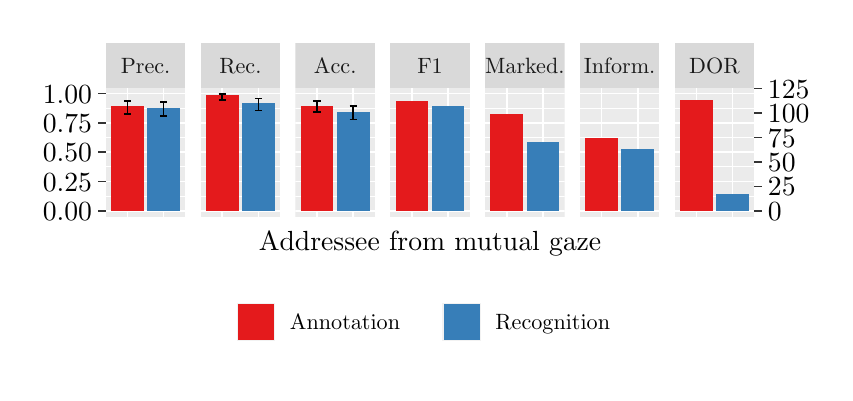
\begin{tikzpicture}[x=1pt,y=1pt]
\definecolor{fillColor}{RGB}{255,255,255}
\path[use as bounding box,fill=fillColor,fill opacity=0.00] (0,0) rectangle (288.00,124.59);
\begin{scope}
\path[clip] (  0.00,  0.00) rectangle (288.00,124.59);
\definecolor{drawColor}{RGB}{255,255,255}
\definecolor{fillColor}{RGB}{255,255,255}

\path[draw=drawColor,line width= 0.6pt,line join=round,line cap=round,fill=fillColor] (  0.00,  0.00) rectangle (288.00,124.59);
\end{scope}
\begin{scope}
\path[clip] ( 28.22, 56.29) rectangle ( 56.98,102.84);
\definecolor{fillColor}{gray}{0.92}

\path[fill=fillColor] ( 28.22, 56.29) rectangle ( 56.98,102.84);
\definecolor{drawColor}{RGB}{255,255,255}

\path[draw=drawColor,line width= 0.3pt,line join=round] ( 28.22, 63.70) --
	( 56.98, 63.70);

\path[draw=drawColor,line width= 0.3pt,line join=round] ( 28.22, 74.30) --
	( 56.98, 74.30);

\path[draw=drawColor,line width= 0.3pt,line join=round] ( 28.22, 84.90) --
	( 56.98, 84.90);

\path[draw=drawColor,line width= 0.3pt,line join=round] ( 28.22, 95.50) --
	( 56.98, 95.50);

\path[draw=drawColor,line width= 0.6pt,line join=round] ( 28.22, 58.40) --
	( 56.98, 58.40);

\path[draw=drawColor,line width= 0.6pt,line join=round] ( 28.22, 69.00) --
	( 56.98, 69.00);

\path[draw=drawColor,line width= 0.6pt,line join=round] ( 28.22, 79.60) --
	( 56.98, 79.60);

\path[draw=drawColor,line width= 0.6pt,line join=round] ( 28.22, 90.20) --
	( 56.98, 90.20);

\path[draw=drawColor,line width= 0.6pt,line join=round] ( 28.22,100.80) --
	( 56.98,100.80);

\path[draw=drawColor,line width= 0.6pt,line join=round] ( 36.07, 56.29) --
	( 36.07,102.84);

\path[draw=drawColor,line width= 0.6pt,line join=round] ( 49.14, 56.29) --
	( 49.14,102.84);
\definecolor{fillColor}{RGB}{228,26,28}

\path[fill=fillColor] ( 30.18, 58.40) rectangle ( 41.95, 96.15);
\definecolor{fillColor}{RGB}{55,126,184}

\path[fill=fillColor] ( 43.26, 58.40) rectangle ( 55.02, 95.57);
\definecolor{drawColor}{RGB}{0,0,0}

\path[draw=drawColor,line width= 0.6pt,line join=round] ( 47.83, 97.68) --
	( 50.45, 97.68);

\path[draw=drawColor,line width= 0.6pt,line join=round] ( 49.14, 97.68) --
	( 49.14, 92.75);

\path[draw=drawColor,line width= 0.6pt,line join=round] ( 47.83, 92.75) --
	( 50.45, 92.75);

\path[draw=drawColor,line width= 0.6pt,line join=round] ( 34.76, 98.09) --
	( 37.37, 98.09);

\path[draw=drawColor,line width= 0.6pt,line join=round] ( 36.07, 98.09) --
	( 36.07, 93.51);

\path[draw=drawColor,line width= 0.6pt,line join=round] ( 34.76, 93.51) --
	( 37.37, 93.51);
\end{scope}
\begin{scope}
\path[clip] ( 62.48, 56.29) rectangle ( 91.25,102.84);
\definecolor{fillColor}{gray}{0.92}

\path[fill=fillColor] ( 62.48, 56.29) rectangle ( 91.25,102.84);
\definecolor{drawColor}{RGB}{255,255,255}

\path[draw=drawColor,line width= 0.3pt,line join=round] ( 62.48, 63.70) --
	( 91.25, 63.70);

\path[draw=drawColor,line width= 0.3pt,line join=round] ( 62.48, 74.30) --
	( 91.25, 74.30);

\path[draw=drawColor,line width= 0.3pt,line join=round] ( 62.48, 84.90) --
	( 91.25, 84.90);

\path[draw=drawColor,line width= 0.3pt,line join=round] ( 62.48, 95.50) --
	( 91.25, 95.50);

\path[draw=drawColor,line width= 0.6pt,line join=round] ( 62.48, 58.40) --
	( 91.25, 58.40);

\path[draw=drawColor,line width= 0.6pt,line join=round] ( 62.48, 69.00) --
	( 91.25, 69.00);

\path[draw=drawColor,line width= 0.6pt,line join=round] ( 62.48, 79.60) --
	( 91.25, 79.60);

\path[draw=drawColor,line width= 0.6pt,line join=round] ( 62.48, 90.20) --
	( 91.25, 90.20);

\path[draw=drawColor,line width= 0.6pt,line join=round] ( 62.48,100.80) --
	( 91.25,100.80);

\path[draw=drawColor,line width= 0.6pt,line join=round] ( 70.33, 56.29) --
	( 70.33,102.84);

\path[draw=drawColor,line width= 0.6pt,line join=round] ( 83.40, 56.29) --
	( 83.40,102.84);
\definecolor{fillColor}{RGB}{228,26,28}

\path[fill=fillColor] ( 64.45, 58.40) rectangle ( 76.21,100.15);
\definecolor{fillColor}{RGB}{55,126,184}

\path[fill=fillColor] ( 77.52, 58.40) rectangle ( 89.29, 97.26);
\definecolor{drawColor}{RGB}{0,0,0}

\path[draw=drawColor,line width= 0.6pt,line join=round] ( 82.09, 99.00) --
	( 84.71, 99.00);

\path[draw=drawColor,line width= 0.6pt,line join=round] ( 83.40, 99.00) --
	( 83.40, 94.68);

\path[draw=drawColor,line width= 0.6pt,line join=round] ( 82.09, 94.68) --
	( 84.71, 94.68);

\path[draw=drawColor,line width= 0.6pt,line join=round] ( 69.02,100.72) --
	( 71.64,100.72);

\path[draw=drawColor,line width= 0.6pt,line join=round] ( 70.33,100.72) --
	( 70.33, 98.52);

\path[draw=drawColor,line width= 0.6pt,line join=round] ( 69.02, 98.52) --
	( 71.64, 98.52);
\end{scope}
\begin{scope}
\path[clip] ( 96.75, 56.29) rectangle (125.51,102.84);
\definecolor{fillColor}{gray}{0.92}

\path[fill=fillColor] ( 96.75, 56.29) rectangle (125.51,102.84);
\definecolor{drawColor}{RGB}{255,255,255}

\path[draw=drawColor,line width= 0.3pt,line join=round] ( 96.75, 63.70) --
	(125.51, 63.70);

\path[draw=drawColor,line width= 0.3pt,line join=round] ( 96.75, 74.30) --
	(125.51, 74.30);

\path[draw=drawColor,line width= 0.3pt,line join=round] ( 96.75, 84.90) --
	(125.51, 84.90);

\path[draw=drawColor,line width= 0.3pt,line join=round] ( 96.75, 95.50) --
	(125.51, 95.50);

\path[draw=drawColor,line width= 0.6pt,line join=round] ( 96.75, 58.40) --
	(125.51, 58.40);

\path[draw=drawColor,line width= 0.6pt,line join=round] ( 96.75, 69.00) --
	(125.51, 69.00);

\path[draw=drawColor,line width= 0.6pt,line join=round] ( 96.75, 79.60) --
	(125.51, 79.60);

\path[draw=drawColor,line width= 0.6pt,line join=round] ( 96.75, 90.20) --
	(125.51, 90.20);

\path[draw=drawColor,line width= 0.6pt,line join=round] ( 96.75,100.80) --
	(125.51,100.80);

\path[draw=drawColor,line width= 0.6pt,line join=round] (104.59, 56.29) --
	(104.59,102.84);

\path[draw=drawColor,line width= 0.6pt,line join=round] (117.66, 56.29) --
	(117.66,102.84);
\definecolor{fillColor}{RGB}{228,26,28}

\path[fill=fillColor] ( 98.71, 58.40) rectangle (110.47, 96.46);
\definecolor{fillColor}{RGB}{55,126,184}

\path[fill=fillColor] (111.78, 58.40) rectangle (123.55, 94.05);
\definecolor{drawColor}{RGB}{0,0,0}

\path[draw=drawColor,line width= 0.6pt,line join=round] (116.36, 96.20) --
	(118.97, 96.20);

\path[draw=drawColor,line width= 0.6pt,line join=round] (117.66, 96.20) --
	(117.66, 91.40);

\path[draw=drawColor,line width= 0.6pt,line join=round] (116.36, 91.40) --
	(118.97, 91.40);

\path[draw=drawColor,line width= 0.6pt,line join=round] (103.28, 98.18) --
	(105.90, 98.18);

\path[draw=drawColor,line width= 0.6pt,line join=round] (104.59, 98.18) --
	(104.59, 94.15);

\path[draw=drawColor,line width= 0.6pt,line join=round] (103.28, 94.15) --
	(105.90, 94.15);
\end{scope}
\begin{scope}
\path[clip] (131.01, 56.29) rectangle (159.77,102.84);
\definecolor{fillColor}{gray}{0.92}

\path[fill=fillColor] (131.01, 56.29) rectangle (159.77,102.84);
\definecolor{drawColor}{RGB}{255,255,255}

\path[draw=drawColor,line width= 0.3pt,line join=round] (131.01, 63.70) --
	(159.77, 63.70);

\path[draw=drawColor,line width= 0.3pt,line join=round] (131.01, 74.30) --
	(159.77, 74.30);

\path[draw=drawColor,line width= 0.3pt,line join=round] (131.01, 84.90) --
	(159.77, 84.90);

\path[draw=drawColor,line width= 0.3pt,line join=round] (131.01, 95.50) --
	(159.77, 95.50);

\path[draw=drawColor,line width= 0.6pt,line join=round] (131.01, 58.40) --
	(159.77, 58.40);

\path[draw=drawColor,line width= 0.6pt,line join=round] (131.01, 69.00) --
	(159.77, 69.00);

\path[draw=drawColor,line width= 0.6pt,line join=round] (131.01, 79.60) --
	(159.77, 79.60);

\path[draw=drawColor,line width= 0.6pt,line join=round] (131.01, 90.20) --
	(159.77, 90.20);

\path[draw=drawColor,line width= 0.6pt,line join=round] (131.01,100.80) --
	(159.77,100.80);

\path[draw=drawColor,line width= 0.6pt,line join=round] (138.85, 56.29) --
	(138.85,102.84);

\path[draw=drawColor,line width= 0.6pt,line join=round] (151.93, 56.29) --
	(151.93,102.84);
\definecolor{fillColor}{RGB}{228,26,28}

\path[fill=fillColor] (132.97, 58.40) rectangle (144.73, 98.05);
\definecolor{fillColor}{RGB}{55,126,184}

\path[fill=fillColor] (146.04, 58.40) rectangle (157.81, 96.40);
\end{scope}
\begin{scope}
\path[clip] (165.27, 56.29) rectangle (194.03,102.84);
\definecolor{fillColor}{gray}{0.92}

\path[fill=fillColor] (165.27, 56.29) rectangle (194.03,102.84);
\definecolor{drawColor}{RGB}{255,255,255}

\path[draw=drawColor,line width= 0.3pt,line join=round] (165.27, 63.70) --
	(194.03, 63.70);

\path[draw=drawColor,line width= 0.3pt,line join=round] (165.27, 74.30) --
	(194.03, 74.30);

\path[draw=drawColor,line width= 0.3pt,line join=round] (165.27, 84.90) --
	(194.03, 84.90);

\path[draw=drawColor,line width= 0.3pt,line join=round] (165.27, 95.50) --
	(194.03, 95.50);

\path[draw=drawColor,line width= 0.6pt,line join=round] (165.27, 58.40) --
	(194.03, 58.40);

\path[draw=drawColor,line width= 0.6pt,line join=round] (165.27, 69.00) --
	(194.03, 69.00);

\path[draw=drawColor,line width= 0.6pt,line join=round] (165.27, 79.60) --
	(194.03, 79.60);

\path[draw=drawColor,line width= 0.6pt,line join=round] (165.27, 90.20) --
	(194.03, 90.20);

\path[draw=drawColor,line width= 0.6pt,line join=round] (165.27,100.80) --
	(194.03,100.80);

\path[draw=drawColor,line width= 0.6pt,line join=round] (173.11, 56.29) --
	(173.11,102.84);

\path[draw=drawColor,line width= 0.6pt,line join=round] (186.19, 56.29) --
	(186.19,102.84);
\definecolor{fillColor}{RGB}{228,26,28}

\path[fill=fillColor] (167.23, 58.40) rectangle (179.00, 93.32);
\definecolor{fillColor}{RGB}{55,126,184}

\path[fill=fillColor] (180.30, 58.40) rectangle (192.07, 83.30);
\end{scope}
\begin{scope}
\path[clip] (199.53, 56.29) rectangle (228.29,102.84);
\definecolor{fillColor}{gray}{0.92}

\path[fill=fillColor] (199.53, 56.29) rectangle (228.29,102.84);
\definecolor{drawColor}{RGB}{255,255,255}

\path[draw=drawColor,line width= 0.3pt,line join=round] (199.53, 63.70) --
	(228.29, 63.70);

\path[draw=drawColor,line width= 0.3pt,line join=round] (199.53, 74.30) --
	(228.29, 74.30);

\path[draw=drawColor,line width= 0.3pt,line join=round] (199.53, 84.90) --
	(228.29, 84.90);

\path[draw=drawColor,line width= 0.3pt,line join=round] (199.53, 95.50) --
	(228.29, 95.50);

\path[draw=drawColor,line width= 0.6pt,line join=round] (199.53, 58.40) --
	(228.29, 58.40);

\path[draw=drawColor,line width= 0.6pt,line join=round] (199.53, 69.00) --
	(228.29, 69.00);

\path[draw=drawColor,line width= 0.6pt,line join=round] (199.53, 79.60) --
	(228.29, 79.60);

\path[draw=drawColor,line width= 0.6pt,line join=round] (199.53, 90.20) --
	(228.29, 90.20);

\path[draw=drawColor,line width= 0.6pt,line join=round] (199.53,100.80) --
	(228.29,100.80);

\path[draw=drawColor,line width= 0.6pt,line join=round] (207.37, 56.29) --
	(207.37,102.84);

\path[draw=drawColor,line width= 0.6pt,line join=round] (220.45, 56.29) --
	(220.45,102.84);
\definecolor{fillColor}{RGB}{228,26,28}

\path[fill=fillColor] (201.49, 58.40) rectangle (213.26, 84.74);
\definecolor{fillColor}{RGB}{55,126,184}

\path[fill=fillColor] (214.57, 58.40) rectangle (226.33, 80.88);
\end{scope}
\begin{scope}
\path[clip] (233.79, 56.29) rectangle (262.55,102.84);
\definecolor{fillColor}{gray}{0.92}

\path[fill=fillColor] (233.79, 56.29) rectangle (262.55,102.84);
\definecolor{drawColor}{RGB}{255,255,255}

\path[draw=drawColor,line width= 0.3pt,line join=round] (233.79, 63.70) --
	(262.55, 63.70);

\path[draw=drawColor,line width= 0.3pt,line join=round] (233.79, 74.30) --
	(262.55, 74.30);

\path[draw=drawColor,line width= 0.3pt,line join=round] (233.79, 84.90) --
	(262.55, 84.90);

\path[draw=drawColor,line width= 0.3pt,line join=round] (233.79, 95.50) --
	(262.55, 95.50);

\path[draw=drawColor,line width= 0.6pt,line join=round] (233.79, 58.40) --
	(262.55, 58.40);

\path[draw=drawColor,line width= 0.6pt,line join=round] (233.79, 69.00) --
	(262.55, 69.00);

\path[draw=drawColor,line width= 0.6pt,line join=round] (233.79, 79.60) --
	(262.55, 79.60);

\path[draw=drawColor,line width= 0.6pt,line join=round] (233.79, 90.20) --
	(262.55, 90.20);

\path[draw=drawColor,line width= 0.6pt,line join=round] (233.79,100.80) --
	(262.55,100.80);

\path[draw=drawColor,line width= 0.6pt,line join=round] (241.64, 56.29) --
	(241.64,102.84);

\path[draw=drawColor,line width= 0.6pt,line join=round] (254.71, 56.29) --
	(254.71,102.84);
\definecolor{fillColor}{RGB}{228,26,28}

\path[fill=fillColor] (235.75, 58.40) rectangle (247.52, 98.59);
\definecolor{fillColor}{RGB}{55,126,184}

\path[fill=fillColor] (248.83, 58.40) rectangle (260.59, 64.57);
\end{scope}
\begin{scope}
\path[clip] ( 28.22,102.84) rectangle ( 56.98,119.09);
\definecolor{fillColor}{gray}{0.85}

\path[fill=fillColor] ( 28.22,102.84) rectangle ( 56.98,119.09);
\definecolor{drawColor}{gray}{0.10}

\node[text=drawColor,anchor=base,inner sep=0pt, outer sep=0pt, scale=  0.80] at ( 42.60,108.21) {Prec.};
\end{scope}
\begin{scope}
\path[clip] ( 62.48,102.84) rectangle ( 91.25,119.09);
\definecolor{fillColor}{gray}{0.85}

\path[fill=fillColor] ( 62.48,102.84) rectangle ( 91.25,119.09);
\definecolor{drawColor}{gray}{0.10}

\node[text=drawColor,anchor=base,inner sep=0pt, outer sep=0pt, scale=  0.80] at ( 76.87,108.21) {Rec.};
\end{scope}
\begin{scope}
\path[clip] ( 96.75,102.84) rectangle (125.51,119.09);
\definecolor{fillColor}{gray}{0.85}

\path[fill=fillColor] ( 96.75,102.84) rectangle (125.51,119.09);
\definecolor{drawColor}{gray}{0.10}

\node[text=drawColor,anchor=base,inner sep=0pt, outer sep=0pt, scale=  0.80] at (111.13,108.21) {Acc.};
\end{scope}
\begin{scope}
\path[clip] (131.01,102.84) rectangle (159.77,119.09);
\definecolor{fillColor}{gray}{0.85}

\path[fill=fillColor] (131.01,102.84) rectangle (159.77,119.09);
\definecolor{drawColor}{gray}{0.10}

\node[text=drawColor,anchor=base,inner sep=0pt, outer sep=0pt, scale=  0.80] at (145.39,108.21) {F1};
\end{scope}
\begin{scope}
\path[clip] (165.27,102.84) rectangle (194.03,119.09);
\definecolor{fillColor}{gray}{0.85}

\path[fill=fillColor] (165.27,102.84) rectangle (194.03,119.09);
\definecolor{drawColor}{gray}{0.10}

\node[text=drawColor,anchor=base,inner sep=0pt, outer sep=0pt, scale=  0.80] at (179.65,108.21) {Marked.};
\end{scope}
\begin{scope}
\path[clip] (199.53,102.84) rectangle (228.29,119.09);
\definecolor{fillColor}{gray}{0.85}

\path[fill=fillColor] (199.53,102.84) rectangle (228.29,119.09);
\definecolor{drawColor}{gray}{0.10}

\node[text=drawColor,anchor=base,inner sep=0pt, outer sep=0pt, scale=  0.80] at (213.91,108.21) {Inform.};
\end{scope}
\begin{scope}
\path[clip] (233.79,102.84) rectangle (262.55,119.09);
\definecolor{fillColor}{gray}{0.85}

\path[fill=fillColor] (233.79,102.84) rectangle (262.55,119.09);
\definecolor{drawColor}{gray}{0.10}

\node[text=drawColor,anchor=base,inner sep=0pt, outer sep=0pt, scale=  0.80] at (248.17,108.21) {DOR};
\end{scope}
\begin{scope}
\path[clip] (  0.00,  0.00) rectangle (288.00,124.59);
\definecolor{drawColor}{RGB}{0,0,0}

\node[text=drawColor,anchor=base east,inner sep=0pt, outer sep=0pt, scale=  1.00] at ( 23.27, 54.96) {0.00};

\node[text=drawColor,anchor=base east,inner sep=0pt, outer sep=0pt, scale=  1.00] at ( 23.27, 65.56) {0.25};

\node[text=drawColor,anchor=base east,inner sep=0pt, outer sep=0pt, scale=  1.00] at ( 23.27, 76.16) {0.50};

\node[text=drawColor,anchor=base east,inner sep=0pt, outer sep=0pt, scale=  1.00] at ( 23.27, 86.75) {0.75};

\node[text=drawColor,anchor=base east,inner sep=0pt, outer sep=0pt, scale=  1.00] at ( 23.27, 97.35) {1.00};
\end{scope}
\begin{scope}
\path[clip] (  0.00,  0.00) rectangle (288.00,124.59);
\definecolor{drawColor}{gray}{0.20}

\path[draw=drawColor,line width= 0.6pt,line join=round] ( 25.47, 58.40) --
	( 28.22, 58.40);

\path[draw=drawColor,line width= 0.6pt,line join=round] ( 25.47, 69.00) --
	( 28.22, 69.00);

\path[draw=drawColor,line width= 0.6pt,line join=round] ( 25.47, 79.60) --
	( 28.22, 79.60);

\path[draw=drawColor,line width= 0.6pt,line join=round] ( 25.47, 90.20) --
	( 28.22, 90.20);

\path[draw=drawColor,line width= 0.6pt,line join=round] ( 25.47,100.80) --
	( 28.22,100.80);
\end{scope}
\begin{scope}
\path[clip] (  0.00,  0.00) rectangle (288.00,124.59);
\definecolor{drawColor}{gray}{0.20}

\path[draw=drawColor,line width= 0.6pt,line join=round] (262.55, 58.40) --
	(265.30, 58.40);

\path[draw=drawColor,line width= 0.6pt,line join=round] (262.55, 67.23) --
	(265.30, 67.23);

\path[draw=drawColor,line width= 0.6pt,line join=round] (262.55, 76.07) --
	(265.30, 76.07);

\path[draw=drawColor,line width= 0.6pt,line join=round] (262.55, 84.90) --
	(265.30, 84.90);

\path[draw=drawColor,line width= 0.6pt,line join=round] (262.55, 93.73) --
	(265.30, 93.73);

\path[draw=drawColor,line width= 0.6pt,line join=round] (262.55,102.56) --
	(265.30,102.56);
\end{scope}
\begin{scope}
\path[clip] (  0.00,  0.00) rectangle (288.00,124.59);
\definecolor{drawColor}{RGB}{0,0,0}

\node[text=drawColor,anchor=base west,inner sep=0pt, outer sep=0pt, scale=  1.00] at (267.50, 54.96) {0};

\node[text=drawColor,anchor=base west,inner sep=0pt, outer sep=0pt, scale=  1.00] at (267.50, 63.79) {25};

\node[text=drawColor,anchor=base west,inner sep=0pt, outer sep=0pt, scale=  1.00] at (267.50, 72.62) {50};

\node[text=drawColor,anchor=base west,inner sep=0pt, outer sep=0pt, scale=  1.00] at (267.50, 81.46) {75};

\node[text=drawColor,anchor=base west,inner sep=0pt, outer sep=0pt, scale=  1.00] at (267.50, 90.29) {100};

\node[text=drawColor,anchor=base west,inner sep=0pt, outer sep=0pt, scale=  1.00] at (267.50, 99.12) {125};
\end{scope}
\begin{scope}
\path[clip] (  0.00,  0.00) rectangle (288.00,124.59);
\definecolor{drawColor}{RGB}{0,0,0}

\node[text=drawColor,anchor=base,inner sep=0pt, outer sep=0pt, scale=  1.00] at (145.39, 43.90) {Addressee from mutual gaze};
\end{scope}
\begin{scope}
\path[clip] (  0.00,  0.00) rectangle (288.00,124.59);
\definecolor{fillColor}{RGB}{255,255,255}

\path[fill=fillColor] ( 64.83,  5.50) rectangle (225.94, 30.95);
\end{scope}
\begin{scope}
\path[clip] (  0.00,  0.00) rectangle (288.00,124.59);
\definecolor{drawColor}{RGB}{255,255,255}
\definecolor{fillColor}{gray}{0.95}

\path[draw=drawColor,line width= 0.6pt,line join=round,line cap=round,fill=fillColor] ( 75.33, 11.00) rectangle ( 89.79, 25.45);
\end{scope}
\begin{scope}
\path[clip] (  0.00,  0.00) rectangle (288.00,124.59);
\definecolor{fillColor}{RGB}{228,26,28}

\path[fill=fillColor] ( 76.04, 11.71) rectangle ( 89.08, 24.74);
\end{scope}
\begin{scope}
\path[clip] (  0.00,  0.00) rectangle (288.00,124.59);
\definecolor{drawColor}{RGB}{255,255,255}
\definecolor{fillColor}{gray}{0.95}

\path[draw=drawColor,line width= 0.6pt,line join=round,line cap=round,fill=fillColor] (149.56, 11.00) rectangle (164.01, 25.45);
\end{scope}
\begin{scope}
\path[clip] (  0.00,  0.00) rectangle (288.00,124.59);
\definecolor{fillColor}{RGB}{55,126,184}

\path[fill=fillColor] (150.27, 11.71) rectangle (163.30, 24.74);
\end{scope}
\begin{scope}
\path[clip] (  0.00,  0.00) rectangle (288.00,124.59);
\definecolor{drawColor}{RGB}{0,0,0}

\node[text=drawColor,anchor=base west,inner sep=0pt, outer sep=0pt, scale=  0.80] at ( 94.79, 15.47) {Annotation};
\end{scope}
\begin{scope}
\path[clip] (  0.00,  0.00) rectangle (288.00,124.59);
\definecolor{drawColor}{RGB}{0,0,0}

\node[text=drawColor,anchor=base west,inner sep=0pt, outer sep=0pt, scale=  0.80] at (169.01, 15.47) {Recognition};
\end{scope}
\end{tikzpicture}
